\documentclass[10pt]{article}
\usepackage[polish]{babel}
\usepackage[utf8]{inputenc}
\usepackage[T1]{fontenc}
\usepackage{graphicx}
\usepackage[export]{adjustbox}
\graphicspath{ {./images/} }
\usepackage{amsmath}
\usepackage{amsfonts}
\usepackage{amssymb}
\usepackage[version=4]{mhchem}
\usepackage{stmaryrd}
\usepackage{hyperref}
\hypersetup{colorlinks=true, linkcolor=blue, filecolor=magenta, urlcolor=cyan,}
\urlstyle{same}
\usepackage{multirow}

\title{KOD }

\author{}
\date{}


\newcommand\Varangle{\mathop{{<\!\!\!\!\!\text{\small)}}\:}\nolimits}

\begin{document}
\maketitle
IMIĘ I NAZWISKO *\\
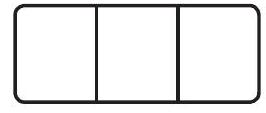
\includegraphics[max width=\textwidth, center]{2024_11_21_a7a52c0c0974ad42b88bg-01}\\
\(\square\)

\begin{itemize}
  \item nieobowiązkowe
\end{itemize}

\section*{PRÓBNY EGZAMIN MATURALNY Z NOWĄ ERĄ MATEMATYKA - POZIOM ROZSZERZONY}
\section*{Instrukcja dla zdającego}
\begin{enumerate}
  \item Sprawdź, czy arkusz egzaminacyjny zawiera \(\mathbf{1 8}\) stron (zadania 1-15). Ewentualny brak stron zgłoś nauczycielowi nadzorującemu egzamin.
  \item Rozwiązania zadań i odpowiedzi zapisz w miejscu na to przeznaczonym.
  \item Pamiętaj, że pominięcie argumentacji lub istotnych obliczeń w rozwiązaniu zadań otwartych może spowodować, że za to rozwiązanie nie otrzymasz pełnej liczby punktów.
  \item Pisz czytelnie. Używaj długopisu/pióra tylko z czarnym tuszem/atramentem.
  \item Nie używaj korektora, a błędne zapisy wyraźnie przekreśl.
  \item Pamiętaj, że zapisy w brudnopisie nie będą oceniane.
  \item Podczas egzaminu możesz korzystać z zestawu wzorów matematycznych, cyrkla i linijki oraz kalkulatora prostego.
  \item Na tej stronie wpisz swój kod oraz imię i nazwisko.
  \item Nie wpisuj żadnych znaków w części przeznaczonej dla osoby sprawdzającej.\\
\(\square\) dysleksja
\end{enumerate}

STYCZEŃ 2018

Czas pracy:\\
180 minut

Liczba punktów\\
do uzyskania: 50

W zadaniach 1.-5. wybierz i zaznacz poprawną odpowiedź.\\
W zadaniu 6. zakoduj wynik w kratkach zamieszczonych pod poleceniem.

Zadanie 1. (0-1)\\
Równanie \(\left|(x+2)^{2}-3\right|=2 a+1 \mathrm{z}\) niewiadomą \(x\) ma dokładnie trzy rozwiązania tylko wtedy, gdy\\
A. \(a=-2\).\\
B. \(a=0\).\\
C. \(a=1\).\\
D. \(a=3\).

Zadanie 2. (0-1)\\
Wskaż przedział, w którym wielomian \(f(x)=x^{3}-6 x^{2}+9 x\) jest funkcją malejącą.\\
A. \(\langle 1,3\rangle\)\\
B. \(\langle 0,4\rangle\)\\
C. \((-\infty, 0)\)\\
D. \((-3,-1)\)

Zadanie 3. \(\mathbf{( 0 - 1 )}\)\\
Nieskończony ciąg liczbowy jest określony wzorem \(a_{n}=\frac{3 n\left(n^{2}-1\right)}{(2 n+1)^{3}}\) dla \(n \geqslant 1\). Wtedy\\
A. \(\lim _{n \rightarrow \infty} a_{n}=3\).\\
B. \(\lim _{n \rightarrow \infty} a_{n}=\frac{3}{2}\).\\
C. \(\lim _{n \rightarrow \infty} a_{n}=\frac{3}{4}\).\\
D. \(\lim _{n \rightarrow \infty} a_{n}=\frac{3}{8}\).

\section*{Zadanie 4. (0-1)}
Funkcja \(f\), której dziedziną jest zbiór \((2, \infty)\), jest określona wzorem: \(f(x)=x+2+\frac{4}{x}+\frac{8}{x^{2}}+\ldots\). Wartość funkcji \(f\) jest równa 8 dla argumentu\\
A. \(\frac{16}{7}\).\\
B. 4 .\\
C. \(4+4 \sqrt{2}\).\\
D. \(10 \frac{2}{3}\).

\section*{Zadanie 5. (0-1)}
Wskaż równanie okręgu, którego obrazem w przesunięciu o wektor \(\vec{u}=[3,-2]\) jest okrąg o równaniu: \(x^{2}+y^{2}-2 x+2 y-2=0\).\\
A. \((x-4)^{2}+(y+3)^{2}=4\)\\
B. \((x+2)^{2}+(y-1)^{2}=2\)\\
C. \((x-3)^{2}+(y+2)^{2}=2\)\\
D. \((x+2)^{2}+(y-1)^{2}=4\)

Zadanie 6. (0-2)\\
W trójkącie ostrokątnym \(A B C \sin \Varangle B A C=\frac{4}{5}\), a \(\sin \Varangle A B C=\frac{2 \sqrt{2}}{3}\). Oblicz \(\cos \Varangle A C B\).\\
W poniższe kratki wpisz kolejno trzy pierwsze cyfry po przecinku rozwinięcia dziesiętnego otrzymanego wyniku.\\
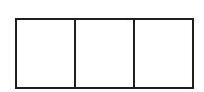
\includegraphics[max width=\textwidth, center]{2024_11_21_a7a52c0c0974ad42b88bg-02}

\section*{BRUDNOPIS (nie podlega ocenie)}
Więcej arkuszy znajdziesz na stronie: \href{http://arkusze.pl}{arkusze.pl}\\

\includegraphics[max width=\textwidth, center]{2024_11_21_a7a52c0c0974ad42b88bg-03}

\begin{center}
\begin{tabular}{|l|l|c|c|c|c|c|c|}
\hline
\multirow{2}{*}{\begin{tabular}{c}
Wypełnia \\
sprawdzający \\
\end{tabular}} & Nr zadania & 1 & 2 & 3 & 4 & 5 & 6 \\
\cline { 2 - 8 }
 & Maks. liczba pkt & 1 & 1 & 1 & 1 & 1 & 2 \\
\cline { 2 - 8 }
 & Uzyskana liczba pkt &  &  &  &  &  &  \\
\hline
\end{tabular}
\end{center}

Zadanie 7. (0-3)\\
W czworokącie \(A B C D\) dane są: \(|A C|=5,|\Varangle B A D|=|\Varangle B C D|=90^{\circ}, \sin \Varangle A B C=\frac{\sqrt{5}}{3}\).\\
Oblicz długość przekątnej \(B D\) tego czworokąta.

Więcej arkuszy znajdziesz na stronie: \href{http://arkusze.pl}{arkusze.pl}\\

\includegraphics[max width=\textwidth, center]{2024_11_21_a7a52c0c0974ad42b88bg-04}

Odpowiedź:

Zadanie 8. (0-3)\\
Udowodnij, że dla każdej liczby rzeczywistej \(x\) prawdziwa jest nierówność:\\
\(x^{4}-4 x^{3}-2 x^{2}+12 x+9 \geqslant 0\).

Więcej arkuszy znajdziesz na stronie: \href{http://arkusze.pl}{arkusze.pl}\\

\includegraphics[max width=\textwidth, center]{2024_11_21_a7a52c0c0974ad42b88bg-05}

\begin{center}
\begin{tabular}{|l|l|c|c|}
\hline
\multirow{2}{*}{\begin{tabular}{c}
Wypełnia \\
sprawdzający \\
\end{tabular}} & Nr zadania & 7 & 8 \\
\cline { 2 - 4 }
 & Maks. liczba pkt & 3 & 3 \\
\cline { 2 - 4 }
 & Uzyskana liczba pkt &  &  \\
\hline
\end{tabular}
\end{center}

Zadanie 9. (0-3)\\
Ciąg \(\left(a_{n}\right)\) jest określony wzorem:\\
\(a_{n}=\frac{1}{\frac{1}{\log _{2}(n+1)}+\frac{1}{\log _{3}(n+1)}+\frac{1}{\log _{4}(n+1)}+\ldots+\frac{1}{\log _{2018}(n+1)}}\) dla \(n \geqslant 1\).\\
Uzasadnij, że wzór ciągu \(\left(a_{n}\right)\) można zapisać w postaci \(a_{n}=\log _{2018!}(n+1)\) i oblicz wartość wyrażenia \(a_{1}+a_{2}+a_{3}+\ldots+a_{2017}\).\\

\includegraphics[max width=\textwidth, center]{2024_11_21_a7a52c0c0974ad42b88bg-06}

Zadanie 10. (0-5)\\
Wyznacz wszystkie liczby rzeczywiste \(x\) spełniające równanie: \(2 \sin ^{2} x-\cos 2 x=1\). Oblicz sumę wszystkich rozwiązań tego równania należących do przedziału \(\langle 0,32 \pi\rangle\).\\

\includegraphics[max width=\textwidth, center]{2024_11_21_a7a52c0c0974ad42b88bg-07}

Odpowiedź:

\begin{center}
\begin{tabular}{|l|l|c|c|}
\hline
\multirow{3}{*}{\begin{tabular}{c}
Wypełnia \\
sprawdzający \\
\end{tabular}} & Nr zadania & 9 & 10 \\
\cline { 2 - 4 }
 & Maks. liczba pkt & 3 & 5 \\
\cline { 2 - 4 }
 & Uzyskana liczba pkt &  &  \\
\hline
\end{tabular}
\end{center}

Zadanie 11. (0-5)\\
Urna zawiera 5 kul ponumerowanych od 1 do 5 . Losowano z niej osiem razy ze zwracaniem po jednej kuli i zapisywano wylosowane numery kolejno, od strony lewej do prawej. Zapisane cyfry utworzyły liczbę ośmiocyfrową. Oblicz prawdopodobieństwo zdarzenia, że w doświadczeniu otrzymamy liczbę parzystą, w której zapisie dziesiętnym znajdą się dokładnie trzy trójki i co najmniej jedna piątka. Wynik podaj w postaci nieskracalnego ułamka zwykłego.\\

\includegraphics[max width=\textwidth, center]{2024_11_21_a7a52c0c0974ad42b88bg-08}\\
Więcej arkuszy znajdziesz na stronie: \href{http://arkusze.pl}{arkusze.pl}\\

\includegraphics[max width=\textwidth, center]{2024_11_21_a7a52c0c0974ad42b88bg-09}

Odpowiedź:

\begin{center}
\begin{tabular}{|l|l|c|}
\hline
\multirow{2}{*}{\begin{tabular}{c}
Wypełnia \\
sprawdzający \\
\end{tabular}} & Nr zadania & 11 \\
\cline { 2 - 3 }
 & Maks. liczba pkt & 5 \\
\cline { 2 - 3 }
 & Uzyskana liczba pkt &  \\
\hline
\end{tabular}
\end{center}

\section*{Zadanie 12. (0-5)}
W ostrosłupie \(A B C S\) podstawa \(A B C\) jest trójkątem równoramiennym o ramionach \(A C\) i \(B C\) długości 4 i kącie między nimi \(30^{\circ}\). Punkt \(E\) - środek krawędzi \(A B\) - jest spodkiem wysokości tego ostrosłupa, a krawędź boczna CS tworzy z podstawą kąt \(60^{\circ}\). Ostrosłup przecięto płaszczyzną przechodzącą przez krawędź \(A B\) i mającą z przeciwległą krawędzią boczną \(C S\) wspólny punkt \(D\) (jak na rysunku). Oblicz pole otrzymanego przekroju, wiedząc, że z podstawą ostrosłupa tworzy on kąt \(75^{\circ}\). Podaj dokładny wynik obliczeń.\\
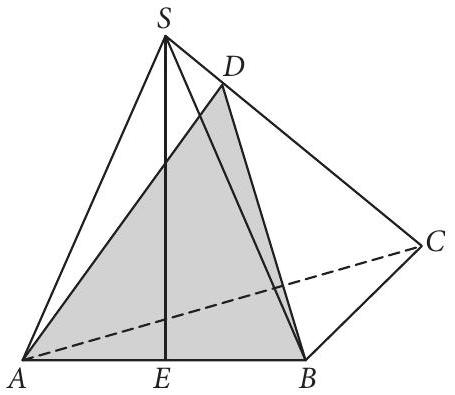
\includegraphics[max width=\textwidth, center]{2024_11_21_a7a52c0c0974ad42b88bg-10}\\

\includegraphics[max width=\textwidth, center]{2024_11_21_a7a52c0c0974ad42b88bg-10(1)}\\
Więcej arkuszy znajdziesz na stronie: \href{http://arkusze.pl}{arkusze.pl}\\

\includegraphics[max width=\textwidth, center]{2024_11_21_a7a52c0c0974ad42b88bg-11}

Odpowiedź:

\begin{center}
\begin{tabular}{|l|l|c|}
\hline
\multirow{2}{*}{\begin{tabular}{c}
Wypełnia \\
sprawdzający \\
\end{tabular}} & Nr zadania & 12 \\
\cline { 2 - 3 }
 & Maks. liczba pkt & 5 \\
\cline { 2 - 3 }
 & Uzyskana liczba pkt &  \\
\hline
\end{tabular}
\end{center}

Zadanie 13. (0-6)\\
Funkcja kwadratowa \(f(x)=(2 m-1) x^{2}-2(m+1) x+m-1\) ma dwa różne miejsca zerowe \(x_{1}, x_{2}\). Wyznacz wszystkie wartości parametru \(m\), dla których odległość między miejscami zerowymi wynosi nie więcej niż 4.

\begin{center}
\begin{tabular}{|c|c|c|c|c|c|c|c|c|c|c|c|c|c|c|c|c|c|c|c|c|c|c|c|c|c|c|c|c|c|}
\hline
 &  &  &  &  &  &  &  &  &  &  &  &  &  &  &  &  &  &  &  &  &  &  &  &  &  &  &  &  &  \\
\hline
 &  &  &  &  &  &  &  &  &  &  &  &  &  &  &  &  &  &  &  &  &  &  &  &  &  &  &  &  &  \\
\hline
 &  &  &  &  &  &  &  &  &  &  &  &  &  &  &  &  &  &  &  &  &  &  &  &  &  &  &  &  &  \\
\hline
 &  &  &  &  &  &  &  &  &  &  &  &  &  &  &  &  &  &  &  &  &  &  &  &  &  &  &  &  &  \\
\hline
 &  &  &  &  &  &  &  &  &  &  &  &  &  &  &  &  &  &  &  &  &  &  &  &  &  &  &  &  &  \\
\hline
 &  &  &  &  &  &  &  &  &  &  &  &  &  &  &  &  &  &  &  &  &  &  &  &  &  &  &  &  &  \\
\hline
 &  &  &  &  &  &  &  &  &  &  &  &  &  &  &  &  &  &  &  &  &  &  &  &  &  &  &  &  &  \\
\hline
 &  &  &  &  &  &  &  &  &  &  &  &  &  &  &  &  &  &  &  &  &  &  &  &  &  &  &  &  &  \\
\hline
 &  &  &  &  &  &  &  &  &  &  &  &  &  &  &  &  &  &  &  &  &  &  &  &  &  &  &  &  &  \\
\hline
 &  &  &  &  &  &  &  &  &  &  &  &  &  &  &  &  &  &  &  &  &  &  &  &  &  &  &  &  &  \\
\hline
 &  &  &  &  &  &  &  &  &  &  &  &  &  &  &  &  &  &  &  &  &  &  &  &  &  &  &  &  &  \\
\hline
 &  &  &  &  &  &  &  &  &  &  &  &  &  &  &  &  &  &  &  &  &  &  &  &  &  &  &  &  &  \\
\hline
 &  &  &  &  &  &  &  &  &  &  &  &  &  &  &  &  &  &  &  &  &  &  &  &  &  &  &  &  &  \\
\hline
 &  &  &  &  &  &  &  &  &  &  &  &  &  &  &  &  &  &  &  &  &  &  &  &  &  &  &  &  &  \\
\hline
 &  &  &  &  &  &  &  &  &  &  &  &  &  &  &  &  &  &  &  &  &  &  &  &  &  &  &  &  &  \\
\hline
 &  &  &  &  &  &  &  &  &  &  &  &  &  &  &  &  &  &  &  &  &  &  &  &  &  &  &  &  &  \\
\hline
 &  &  &  &  &  &  &  &  &  &  &  &  &  &  &  &  &  &  &  &  &  &  &  &  &  &  &  &  &  \\
\hline
 &  &  &  &  &  &  &  &  &  &  &  &  &  &  &  &  &  &  &  &  &  &  &  &  &  &  &  &  &  \\
\hline
 &  &  &  &  &  &  &  &  &  &  &  &  &  &  &  &  &  &  &  &  &  &  &  &  &  &  &  &  &  \\
\hline
 &  &  &  &  &  &  &  &  &  &  &  &  &  &  &  &  &  &  &  &  &  &  &  &  &  &  &  &  &  \\
\hline
 &  &  &  &  &  &  &  &  &  &  &  &  &  &  &  &  &  &  &  &  &  &  &  &  &  &  &  &  &  \\
\hline
 &  &  &  &  &  &  &  &  &  &  &  &  &  &  &  &  &  &  &  &  &  &  &  &  &  &  &  &  &  \\
\hline
 &  &  &  &  &  &  &  &  &  &  &  &  &  &  &  &  &  &  &  &  &  &  &  &  &  &  &  &  &  \\
\hline
 &  &  &  &  &  &  &  &  &  &  &  &  &  &  &  &  &  &  &  &  &  &  &  &  &  &  &  &  &  \\
\hline
 &  &  &  &  &  &  &  &  &  &  &  &  &  &  &  &  &  &  &  &  &  &  &  &  &  &  &  &  &  \\
\hline
 &  &  &  &  &  &  &  &  &  &  &  &  &  &  &  &  &  &  &  &  &  &  &  &  &  &  &  &  &  \\
\hline
 &  &  &  &  &  &  &  &  &  &  &  &  &  &  &  &  &  &  &  &  &  &  &  &  &  &  &  &  &  \\
\hline
 &  &  &  &  &  &  &  &  &  &  &  &  &  &  &  &  &  &  &  &  &  &  &  &  &  &  &  &  &  \\
\hline
 &  &  &  &  &  &  &  &  &  &  &  &  &  &  &  &  &  &  &  &  &  &  &  &  &  &  &  &  &  \\
\hline
 &  &  &  &  &  &  &  &  &  &  &  &  &  &  &  &  &  &  &  &  &  &  &  &  &  &  &  &  &  \\
\hline
 &  &  &  &  &  &  &  &  &  &  &  &  &  &  &  &  &  &  &  &  &  &  &  &  &  &  &  &  &  \\
\hline
 &  &  &  &  &  &  &  &  &  &  &  &  &  &  &  &  &  &  &  &  &  &  &  &  &  &  &  &  &  \\
\hline
 &  &  &  &  &  &  &  &  &  &  &  &  &  &  &  &  &  &  &  &  &  &  &  &  &  &  &  &  &  \\
\hline
 &  &  &  &  &  &  &  &  &  &  &  &  &  &  &  &  &  &  &  &  &  &  &  &  &  &  &  &  &  \\
\hline
 &  &  &  &  &  &  &  &  &  &  &  &  &  &  &  &  &  &  &  &  &  &  &  &  &  &  &  &  &  \\
\hline
 &  &  &  &  &  &  &  &  &  &  &  &  &  &  &  &  &  &  &  &  &  &  &  &  &  &  &  &  &  \\
\hline
 &  &  &  &  &  &  &  &  &  &  &  &  &  &  &  &  &  &  &  &  &  &  &  &  &  &  &  &  &  \\
\hline
 &  &  &  &  &  &  &  &  &  &  &  &  &  &  &  &  &  &  &  &  &  &  &  &  &  &  &  &  &  \\
\hline
 &  &  &  &  &  &  &  &  &  &  &  &  &  &  &  &  &  &  &  &  &  &  &  &  &  &  &  &  &  \\
\hline
 &  &  &  &  &  &  &  &  &  &  &  &  &  &  &  &  &  &  &  &  &  &  &  &  &  &  &  &  &  \\
\hline
 &  &  &  &  &  &  &  &  &  &  &  &  &  &  &  &  &  &  &  &  &  &  &  &  &  &  &  &  &  \\
\hline
 &  &  &  &  &  &  &  &  &  &  &  &  &  &  &  &  &  &  &  &  &  &  &  &  &  &  &  &  &  \\
\hline
\end{tabular}
\end{center}

Więcej arkuszy znajdziesz na stronie: \href{http://arkusze.pl}{arkusze.pl}\\

\includegraphics[max width=\textwidth, center]{2024_11_21_a7a52c0c0974ad42b88bg-13}

Odpowiedź:

\begin{center}
\begin{tabular}{|l|l|c|}
\hline
\multirow{2}{*}{\begin{tabular}{c}
Wypełnia \\
sprawdzający \\
\end{tabular}} & Nr zadania & 13 \\
\cline { 2 - 3 }
 & Maks. liczba pkt & 6 \\
\cline { 2 - 3 }
 & Uzyskana liczba pkt &  \\
\hline
\end{tabular}
\end{center}

Zadanie 14. (0-6)\\
Wyznacz równania wszystkich wspólnych stycznych do paraboli o równaniu \(y=\frac{1}{2} x^{2}\) i okręgu\\
o równaniu \(x^{2}+\left(y+\frac{5}{2}\right)^{2}=2\).

Więcej arkuszy znajdziesz na stronie: \href{http://arkusze.pl}{arkusze.pl}\\

\includegraphics[max width=\textwidth, center]{2024_11_21_a7a52c0c0974ad42b88bg-14}\\
Więcej arkuszy znajdziesz na stronie: \href{http://arkusze.pl}{arkusze.pl}\\

\includegraphics[max width=\textwidth, center]{2024_11_21_a7a52c0c0974ad42b88bg-15}

Odpowiedź:

\begin{center}
\begin{tabular}{|l|l|c|}
\hline
\multirow{2}{*}{\begin{tabular}{c}
Wypełnia \\
sprawdzający \\
\end{tabular}} & Nr zadania & 14 \\
\cline { 2 - 3 }
 & Maks. liczba pkt & 6 \\
\cline { 2 - 3 }
 & Uzyskana liczba pkt &  \\
\hline
\end{tabular}
\end{center}

Zadanie 15. (0-7)\\
Prosta o równaniu \(y=a^{2} x+3 a\) przecina hiperbolę o równaniu \(y=\frac{4}{x} \mathrm{w}\) dwóch punktach, \(A\) i \(B\). Wyraź długość odcinka \(A B\) w zależności od wartości parametru \(a<0\). Wyznacz równanie prostej, która przecina opisaną w zadaniu hiperbolę tak, aby długość odcinka \(A B\) była najmniejsza.

Więcej arkuszy znajdziesz na stronie: \href{http://arkusze.pl}{arkusze.pl}\\

\includegraphics[max width=\textwidth, center]{2024_11_21_a7a52c0c0974ad42b88bg-16}\\
Więcej arkuszy znajdziesz na stronie: \href{http://arkusze.pl}{arkusze.pl}\\

\includegraphics[max width=\textwidth, center]{2024_11_21_a7a52c0c0974ad42b88bg-17}

Odpowiedź:

\begin{center}
\begin{tabular}{|l|l|c|}
\hline
\multirow{2}{*}{\begin{tabular}{c}
Wypełnia \\
sprawdzający \\
\end{tabular}} & Nr zadania & 15 \\
\cline { 2 - 3 }
 & Maks. liczba pkt & 7 \\
\cline { 2 - 3 }
 & Uzyskana liczba pkt &  \\
\hline
\end{tabular}
\end{center}

\section*{BRUDNOPIS (nie podlega ocenie)}
Więcej arkuszy znajdziesz na stronie: \href{http://arkusze.pl}{arkusze.pl}\\

\includegraphics[max width=\textwidth, center]{2024_11_21_a7a52c0c0974ad42b88bg-18}


\end{document}